\chapter{Data-driven Landscapes of Colon Epithelial Plasticity}
\label{05vr}

\newpage
\section{Introduction}

More than 60 years ago, Conrad H. Waddington illustrated the process of an epigenetic landscape where pluripotent cells would roll down into valleys of terminally differentiated states~\cite{ch_waddington_waddington_1957}. Albeit a powerful image of developmental biology, his effort and subsequent ones since then have mostly been of a rather subjective and artistic nature. However, reconstructing such landscapes from real biological data is not an untenable task anymore, as \emph{omic} profiles from single-cells can be embedded together and mapped onto a 3D space sculpted by cellular pluripotency metrics \cite{chen_single-cell_2019}.

However, none of those methods appear to leverage embeddings able to capture transitional processes and global structure. Furthermore, such a Waddington-like landscape would need to be informed by features at multiple levels: with a coarse feature informing overall elevation, and local information determining the presence of troughs and valleys, thus shaping the repertoire of likely downhill transitions.

Here I propose a novel method to generate such data-driven Waddington-like landscapes using; 1) embeddings that capture global structure (PHATE \cite{moon_visualizing_2019}), 2) a cellular pluripotency metric to derive coarse landscape elevation (CCAT \cite{teschendorff_single-cell_2017}), and 3) RNA velocity metrics to capture local transciptomic changes (scvelo \cite{bergen_generalizing_2020}) that inform state accessibility (Figure \ref{fig:5land}A).

This work has been published as part of Qin \& Cardoso Rodriguez \emph{et al.}~\cite{cardoso_rodriguez_single-cell_2023}, and the code to compute the VR score and generate the landscapes is publicly available as a Jupyter Notebook on \url{github.com/TAPE-Lab/Qin-CardosoRodriguez-et-al/blob/main/Figure7_S7/Landscape.ipynb}. 

\section{The Valley-Ridge Score}

\begin{figure}
    \centering
    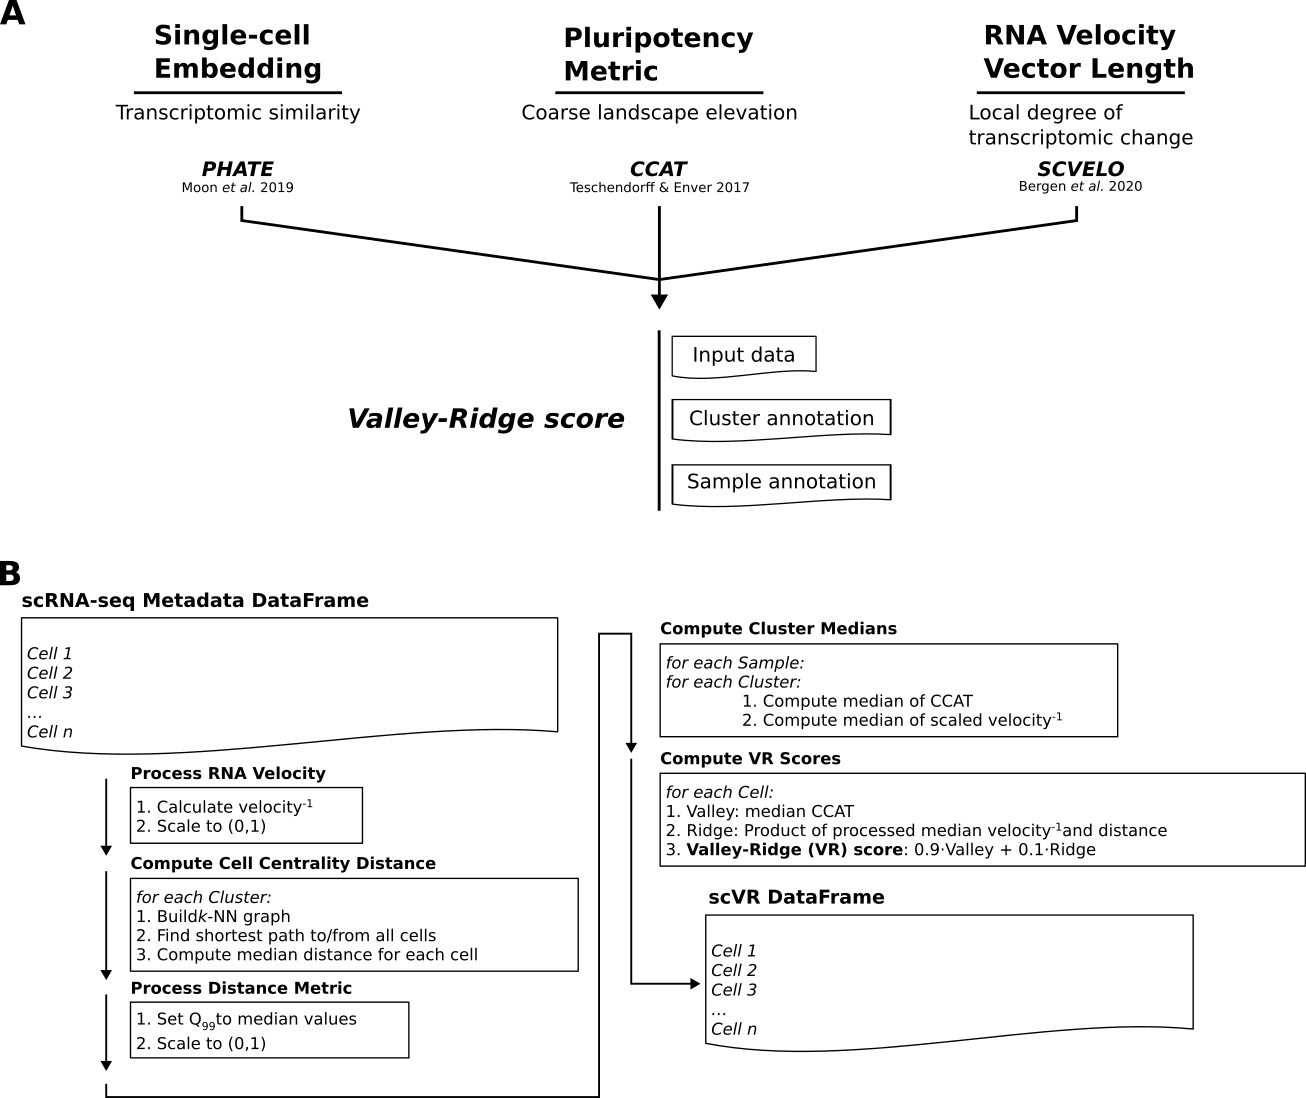
\includegraphics{05vr/figs/5VR_score.png}
    \caption{\textbf{Workflow for Calculating VR Scores from scRNA-seq Data}. \textbf{A)} \acrshort{vr} scores leverage a low-dimensional embedding and are computed from pluripotency and RNA velocity metrics. \textbf{B)} Computation of \acrshort{vr} scores incorporates  global and local components as a weighted sum. \acrshort{vr}, \acrlong{vr}. Q\textsubscript{99}, 99\textsuperscript{th} quantile.}
    \label{fig:5score}
\end{figure}

Following with the geographical analogy, PHATE space acts as the \emph{longitude} and \emph{latitude} coordinates whereas we need to define a new metric that combines both CCAT scores and RNA velocity vector lengths. This metric has been called the Valley-Ridge (VR) score, in reference of its two components that respectively inform macro-level and hyper-local features of the landscape (Figure \ref{fig:5land}A).

While these two metrics have already been discussed previously in this work, here is a small summary of what they entail. CCAT has been defined as an estimate for a cell's Signalling Entropy Rate, which has been shown to be a robust metric for cellular pluripotency \cite{teschendorff_single-cell_2017,chen_single-cell_2019,senra_origins_2022}. RNA velocity vector lengths are the modulus of the inferred RNA velocity vectors as determined by a cell's ratio of spliced and unspliced mRNA, thus measuring the overall rate of transcriptomic change undergone by a cell.

Detailed information on the definition and computation of the VR score can be found in Chapter \ref{02methods}. In brief, the VR score is a cellular metric computed on a per sample and cluster labels and is defined as the weighted sum of the two components: CCAT signalling-entropy~\cite{teschendorff_single-cell_2017} and RNA velocity vector length~\cite{bergen_generalizing_2020} (Figure \ref{fig:5land}B). 
At a cluster's centre, the VR score is solely determined by the median CCAT. However, the VR scores at the cluster periphery are augmented by weighting the inverse of RNA velocity component and the scaled distance from the cluster centre to model rates of local transcriptional change. We use the inverse of the velocity vector length so that transitions substantiated by high RNA velocities do not locally increase landscape elevation at a cluster's boundary, with the opposite happening for low velocity cells.

This method thus reconstructs a data-driven estimate of Waddington-like landscapes where the overall altitude captures the differentiation potential of a cell population, with the \acrlong{vr} topology delineating local plasticity and cell-state availability. 

\section{Landscapes of Colonic Epithelia Cell-Fate Plasticity}

Having been described in Chapter \ref{04seq} and in Qin \& Cardoso Rodriguez \emph{et al.}, the heterocellular murine colonic organoid system represents a suitable candidate to test the VR landscapes. 
This system consists of colon epithelia organoids increasingly accumulating canonical CRC oncogenic mutations, and with various combinations of microenvironmental perturbations including a stromal component (Figure \ref{fig:5land}A).

The cellular dynamics of this system suggest stromal cues polarise colonic epithelia towards a slow-cycling \acrshort{revcsc} state, comprising lower pluripotency potential than other stem states. There is also some loss of terminally differentiated states by stromal cues, especially around the absorptive compartment, but this de-differentiation was not as pronounced as in CRC organoids.
Oncogenic mutations polarise epithelia to the proliferative and highly pluripotent (as determined by CCAT) \acrshort{procsc} state. Furthermore, RNA velocity vector lengths in CRC organoids were greatly reduced when compared to the other genotypes (Figure \ref{fig:4dyn}C-D), suggesting that normal transitional processes within the epithelia are impeded by oncogenic mutations.
The VR score is a way of visualising all of these processes at once by generating a purely data-driven VR landscape reminiscent of Waddington own's drawing.

\begin{figure}[h]
    \centering
    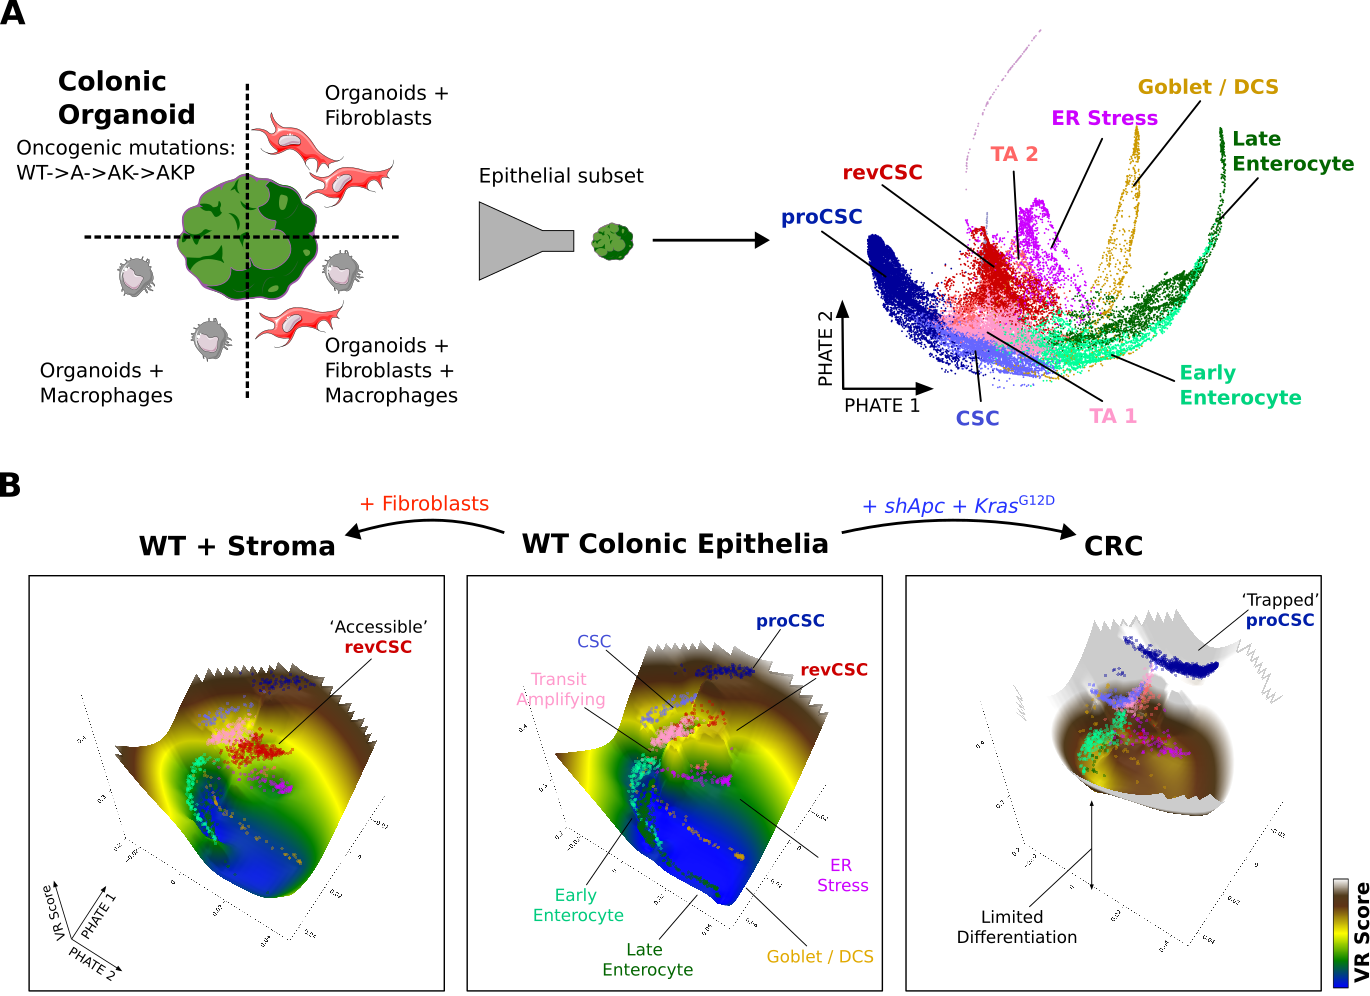
\includegraphics{05vr/figs/5VR_landscape.png}
    \caption{\textbf{Fibroblast- and Oncogene-driven Waddington-like Single-cell Landscapes.} \textbf{A)} Epithelial cells from the heterocellular CRC organoid model system are used to compute \acrshort{vr} scores. \textbf{B)} Integrating PHATE and Valley-Ridge (VR) score enables Waddington-like landscapes of scRNA-seq data, illustrating processes of \acrshort{csc} polarisation. Landscape colour denotes \acrshort{vr} elevation, dot colours represent epithelial clusters.}
     % Landscapes illustrate how WT epithelia differentiate from high signalling-entropy stem cells, through TA cells, into secretory and absorptive cells. Fibroblasts enable WT epithelia to access revCSC while retaining secretory and absorptive differentiation. In contrast, \textit{shApc} and \textit{Kras\textsuperscript{G12D/+}} limit differentiation and trap cells in the proCSC state.
    \label{fig:5land}
\end{figure}

When WT colonic epithelia are projected onto this embedding, stem cells occupy high positions in the landscape, with TA cells descending into a central valley before diverging into terminally differentiated secretory and absorptive cells (Figure \ref{fig:5land}B). When WT epithelia communicate with fibroblasts, the TA valley erodes as cells access revCSC (Figure \ref{fig:5land}B). In contrast, CRC mutations \textit{shApc} and \textit{Kras\textsuperscript{G12D/+}} re-sculpt the entire landscape, trapping most cells in the proCSC fate by restricting their differentiation potential (Figure \ref{fig:5land}B). 

This landscape projection exemplifies the VR score profile of cellular states such as proCSC, which are highly pluripotent (Figure \ref{fig:4dyn}B), yet static in terms of rate of transcriptional change (Figure \ref{fig:4dyn}C). proCSC sates appear as high elevation tarn-like features, surrounded by an obstructive ridge that symbolises the low likelihood of transition towards surrounding states. VR landscapes therefore enable us to visualise how proCSC are a stem cell (high in Waddington space) that rarely differentiate (trapped in a tarn). 

See Chapter \ref{02methods} for details on the methods used to interpolate the VR scores into a surface and the pipeline to generate the VR landscapes (Figure \ref{fig:2land}).

\newpage
\section{Conclusions}

The VR score presented here synthesises two orthogonal metrics (signalling entropy rate and transcriptomic rate of change) that when combined are very useful in visualising transitional processes and plasticity of a system. The multi-scale nature of the its components, with CCAT determining coarser cluster-level features and RNA velocity vector lengths more local inter-cluster transitions, proves useful when reconstructing data-driven Waddington-like landscapes. 

When applied to murine organoid perturbation system described in Chapter \ref{04seq}, the VR landscapes depict a picture of a shared differentiation that can be traversed through cell-extrinsic ligands or cell-intrinsic oncogenic mutations. In particular, the increased availability of \acrshort{revcsc} in the presence of stromal ligands (Figure \ref{fig:4da}) can also be observed on the VR landscapes (Figure \ref{fig:5land}B). Furthermore, the collapse of stromal-to-epithelial communication in cancer organoids (Figure \ref{fig:4cc}A) and their lack of \acrshort{revcsc} polarisation (Figure \ref{fig:4da}C) is reflected in the tarn-like topology of the AK VR landscapes, where the bulk of the organoid appears trapped in the \acrshort{procsc} state.

By combining the VR score computation and landscape projection into a single easy to use notebook, I have laid the foundation towards future packaging and deployment of this tool as an interactive service. By the name of VRland, this tool is currently available as an annotated Jupyter Notebook in the code repository for Qin \& Cardoso Rodriguez \emph{et al.}~\cite{cardoso_rodriguez_single-cell_2023} (\href{www.github.com/TAPE-Lab/Qin-CardosoRodriguez-et-al}{github.com/TAPE-Lab/Qin-CardosoRodriguez-et-al}).
